\documentclass[11pt]{article}

\usepackage{a4wide}
\usepackage{amsmath,amssymb}
\usepackage[english]{babel}
\usepackage{enumitem}
\usepackage{float}
\usepackage{graphicx}
\usepackage[utf8]{inputenc}
\usepackage{listings}
\usepackage{multicol}
\usepackage{tikz}

%========== DEFINITIONS & MACROS ==========%

\definecolor{comment}{rgb}		{0.38, 0.62, 0.38}
\definecolor{keyword}{rgb}		{0.10, 0.10, 0.81}
\definecolor{identifier}{rgb}	{0.00, 0.00, 0.00}
\definecolor{string}{rgb}		{0.50, 0.50, 0.50}

\newcommand{\secref}[1]{see section \ref{#1} on page \pageref{#1}}
\newcommand{\appref}[1]{see appendix \ref{#1} on page \pageref{#1}}
\newcommand{\txtref}[2][]{see {\it #1} \ref{#2} on page \pageref{#2}}
\newcommand{\code}[1]{{\tt #1}}
\newcommand{\file}[1]{{\tt #1}}
\newcommand{\imp}{\rightarrow}
\newcommand{\norm}[1]{\lVert#1\rVert}
\newcommand{\unit}[1]{\frac{#1}{\norm{#1}}}

\setdescription{leftmargin=\parindent, labelindent=\parindent}

\lstset
{
    language=C++,
	% general settings
	numbers=left,
	frame=single,
	basicstyle=\footnotesize\ttfamily,
	tabsize=2,
	breaklines=true,
	% syntax highlighting
	commentstyle=\color{comment},
	keywordstyle=\color{keyword},
	identifierstyle=\color{identifier},
	stringstyle=\color{string},
}


\title
{
    {\Large Individual Assignment 3} \\
    Introduction to Computer Graphics
}

\author
{
    Casper B. Hansen \\
    University of Copenhagen \\
    Department of Computer Science \\
    {\tt fvx507@alumni.ku.dk}
}

\date{last revision \today}

\begin{document}

\clearpage\maketitle\vspace{1in}
\begin{multicols}{2}
    \begin{abstract}
        We will discuss the concept of projections from world coordinates onto
        a surface, for our purposes to produce a projection onto a computer
        screen. We begin by defining eye coordinates, a projection plane and
        a look-through window. With these definitions we proceed by looking at
        how we can produce a parallel projection of objects whose points are
        given in an arbitrary world coordinate system. Implementation of the
        parallel and perspective projections are shown and discussed briefly.
        
        The reader is not expected to have any prior knowledge of the material
        presented. For the code the reader is expected to have some basic
        understanding of linear algebra  and the C++ language.
    \end{abstract}
    \vfill\columnbreak\tableofcontents\vfill
\end{multicols}
\thispagestyle{empty}\newpage

\section{Introductory}
We want to visualize objects whose coordinates are defined by the {\it World
Coordinate System} as though through a camera. That is, we want some amount of
control over the view into this world. Camera's are much like objects in and
of themselves (i.e. they have position and rotation), but they also have some
properties that defines the lense, which affects the image a camera produces.
These are the properties we will be discussing, and specifically we will be
looking to make use of these properties to transform an arbitrary view volume
into the canonical parallel view volume.

\subsection{Eye Coordinate System}
\label{sec:intro|sub:eye-coord-sys}
Let us define what is known as an {\it Eye Coordinate System}. Firstly, an eye
has a position, this is where our {\it ``camera''} will be looking from. Also,
we must establish some form of restriction on what the camera can
{\it ``see''}, for this we will introduce the notion of a projection plane,
with which lines from object coordinates to the viewer eye form points
intersecting with the projection plane. This will be our {\it ``window''} into
the world.

We define the projection plane in the {\it World Coordinate System} by a
{\it View Reference Point} ({\bf VRP}, which is a point on the projection
plane. The point alone gives us nothing more than a position. Adding a {\it
View Plane Normal} ({\bf VPN}) gives the plane its orientation. Likewise, the
camera viewing the world through this projection plane must also establish
some orientation, this is achieved by the {\it View Up Vector} ({\bf VUP}).

The {\it Eye Coordinate System} $Eye(u, v, n)^T$ is then defined as such
\begin{align}
    n = \unit{VPN} \qquad
    u = \unit{VUP \times VNP} \qquad
    v = \unit{VPN \times (VUP \times VPN)}
\end{align}

All of these vectors are divided by their length in order to ensure that these
become unit vectors (i.e. vectors whose magnitude is 1). The $n$ vector points
in the direction of the {\bf VPN}. The $v$ vector is perpendicular to vectors
{\bf VPN} and {\bf VUP}, making it point along the projection plane. The $u$
vector runs along the projection plane perpendicular to the $v$ vector, which
effectively defines the opposing axis.

\subsection{The Window}
\label{sec:intro|sub:window}
Now that we have the {\it Eye Space Coordinates} and a projection plane, we
can define what will be the window on the projection plane through which our
camera will be looking. Since the window will be lying on the projection plane
we simply need to delimit an area within this plane. We do so by defining two
points in the plane; $(u_{min}, v_{min})$ denoting the lower-left, and
$(u_{max}, v_{max})$ denoting the upper-right corners of the window. Taking
the average of the individual components yields the window center
({\bf CW}\footnote{Note that the points {\bf CW} and {\bf VRP} need not
coincide}). That is $CW = (\frac{u_{min} + u_{max}}{2}, \frac{v_{min} +
v_{max}}{2})$.

\subsection{Projection}
\label{sec:intro|sub:projection}
When we define the projection, it is necessary to decide what kind of
projection; orthographic, parallel, perspective, etc. For perspective
projections a fourth point is needed, namely the {\it Projection Reference
Point} ({\bf PRP}), which in relation to the {\bf VRP} defines the {\it
Direction Of Projection} ({\bf DOP}). We can compute this by $DOP = PRP - CW$.

The {\bf DOP} defines the kind of projection we are performing; the projection
is called a perspective projection iff. {\bf PRP} is a finite point.
Contrarily, the projection is called a parallel projection iff. {\bf PRP} is
at infinity. In the case of orthographic projection, obviously points are
projected from the world coordinate system along {\bf VPN} onto the projection
plane --- in order to transform world coordinates into the canonical
orthographic view volume this is simply a matter of removing the depth
coordinate $z$.

\subsection{View Volumes}
\label{sec:intro|sub:view-volumes}
A view volume $V$ is a bounded box within which objects can be viewed, if not
obscurred by other objects in front. As such $V \subset \mathbb{R}^3$. In
example, for a perspective projection the view volume would be a
pyramid-shaped boundary box. It is this view volume we wish to transform into
the canonical parallel view volume. It should be noted that for view volumes
we usually also declare a delimiters for near and far planes, denoting how far
and close our camera can see objects.

\section{Canonical Parallel View Volume}
\label{sec:canonical-parallel-view-volume}
Having defined the principles on which we have built the notion of a camera
thus far, we will now use these to transform world coordinates into what is
known as the {\it Canonical Parallel View Volume}, which produces a parallel
projection matrix.

\subsection{Translate to the origin}
\label{sec:canonical-parallel-view-volume|sub:translate-to-origin}
First, we translate the {\bf VRP} to the origin. This is quite simple, we
multiply by a translation matrix containing the negated coordinates of
{\bf VRP}.
\begin{align}
    T(-VRP) &=
    \begin{bmatrix}
        1 & 0 & 0 & -vrp_x \\
        0 & 1 & 0 & -vrp_y \\
        0 & 0 & 1 & -vrp_z \\
        0 & 0 & 0 & 1
    \end{bmatrix}
\end{align}

\subsection{Rotate to align}
\label{sec:canonical-parallel-view-volume|sub:rotate-to-align}
Having the {\bf VRP} at the origin, we must now ensure that the eye coordinate
axis align with the world. We do this by calculating the unit vectors $u$, $v$
and $n$ (\secref{sec:intro|sub:eye-coord-sys}), and then rotate them to line
them up with the world axis. This is done by the following rotation matrix.
\begin{align}
    R &=
    \begin{bmatrix}
        r_{1x} & r_{2x} & r_{3x} \\
        r_{1y} & r_{2y} & r_{3y} \\
        r_{1z} & r_{2z} & r_{3z}
    \end{bmatrix}
\end{align}
Where the rotation row vectors are given, as mentioned, by the unit vectors
$u$, $v$ and $n$. That is,
\begin{align}
    R_z^T &= (r_{1z}, r_{2z}, r_{3z}) = \unit{VPN} \\
    R_x^T &= (r_{1x}, r_{2x}, r_{3x}) = \unit{VUP \times R_z} \\
    R_y^T &= (r_{1y}, r_{2y}, r_{3y}) = \unit{R_z \times R_x}
\end{align}

\subsection{Shear to parallel projection}
\label{sec:canonical-parallel-view-volume|sub:shear-to-parallel}
Being at the origin and having oriented ourselves correctly, we can now start
deforming the world by shearing, such that the direction of projection becomes
parallel to the $Z$-axis.

To do this, we must first do a bit of arithmetic. We need to solve for $sh_x$
and $sh_y$ in the shear matrix.
\begin{align}
    Sh_{par} &=
    \begin{bmatrix}
        1 & 0 & sh_x & 0 \\
        0 & 1 & sh_y & 0 \\
        0 & 0 & 1 & 0 \\
        0 & 0 & 0 & 1
    \end{bmatrix}
\end{align}

We know that $DOP = PRP - CW = (dop_u, dop_v, dop_n, 0)^T$, and we want the
above shear transformation matrix to produce $DOP' = Sh_{par}DOP = (0, 0,
dop_n, 0)^T$.

If we write up the equation, this is what we get
\begin{align}
    \begin{bmatrix}
        1 & 0 & sh_x & 0 \\
        0 & 1 & sh_y & 0 \\
        0 & 0 & 1 & 0 \\
        0 & 0 & 0 & 1
    \end{bmatrix}
    \begin{bmatrix}
        dop_u \\
        dop_v \\
        dop_n \\
        0
    \end{bmatrix}
    &=
    \begin{bmatrix}
        dop_u + sh_x dop_n \\
        dop_v + sh_y dop_n \\
        dop_n \\
        0
    \end{bmatrix}
    =
    \begin{bmatrix}
        0 \\
        0 \\
        dop_n \\
        0
    \end{bmatrix}
\end{align}
the solution to which is
\begin{align}
    sh_x = -\frac{dop_u}{dop_n} \\
    sh_y = -\frac{dop_v}{dop_n}
\end{align}
Substituting this into our shear transformation matrix, we get that
\begin{align}
    Sh_{par} &=
    \begin{bmatrix}
        1 & 0 & -\frac{dop_u}{dop_n} & 0 \\
        0 & 1 & -\frac{dop_v}{dop_n} & 0 \\
        0 & 0 & 1 & 0 \\
        0 & 0 & 0 & 1
    \end{bmatrix}
\end{align}
with which we can multiply onto our transformations, effectively shearing such
that the direction of projection becomes parallel to the $Z$-axis.

\subsection{Final translation and scale}
\label{sec:canonical-parallel-view-volume|sub:translate-and-scale}
Finally, we translate yet again in order to bring near clipping plane to line
up with the $XY$-plane, and place {\bf CW} at the origin. In order to bring
the near clipping plane into alignment with the $XY$-plane we simply need to
translate by $-near$ on the $z$-axis, and likewise to put {\bf CW} at the
origin we simply need to translate by $-cw_u$ on the $X$-axis and $-cw_v$ on
the $Y$-axis. This yields the following translation matrix.
\begin{align}
    T_{par} &=
    \begin{bmatrix}
        1 & 0 & 0 & -cw_u \\
        0 & 1 & 0 & -cw_v \\
        0 & 0 & 1 & -near \\
        0 & 0 & 0 & 1
    \end{bmatrix}
    &=
    \begin{bmatrix}
        1 & 0 & 0 & -\frac{u_{min} + u_{max}}{2} \\
        0 & 1 & 0 & -\frac{v_{min} + v_{max}}{2} \\
        0 & 0 & 1 & -near \\
        0 & 0 & 0 & 1
    \end{bmatrix}
\end{align}
Note that the right-hand side has been expanded according to the definition of
{\bf CW} discussed earlier (\secref{sec:intro|sub:window}).

Following this translation we scale the current condition of the view volume
such that it gets the proportions $[-1, 1]_X \times [-1, 1]_Y \times
[0, -1]_Z$. We do this by multiplying with the following scale transformation
matrix.
\begin{align}
    S_{par} &=
    \begin{bmatrix}
        \frac{2}{u_{max} - u_{min}} & 0 & 0 & 0 \\
        0 & \frac{2}{v_{max} - v_{min}} & 0 & 0 \\
        0 & 0 & \frac{1}{F - B} & 0 \\
        0 & 0 & 0 & 1
    \end{bmatrix}
\end{align}
Which effectively brings us to the final matrix and the transformation is
completed, the result of which is called {\it The Canonical Parallel View
Volume}.
\begin{align}
    N_{par} = S_{par} \cdot T_{par} \cdot Sh_{par} \cdot R \cdot T(-VRP)
\end{align}
The entirety of the transformation is given by the equation above.

\newpage
\section{Implementation}
\label{sec:implementation}
In my implementation of the projection transformation I have a \code{Camera}
class the definition of which is shown below, containing all of the points of
vectors defined for the eye coordinate system
(\secref{sec:intro|sub:eye-coord-sys}) on lines 25--27, as well as a
projection reference point (\secref{sec:intro|sub:projection}) on line 28. It
also contains the window boundaries (\secref{sec:intro|sub:window}) on lines
30--31, as well as the near and far view volume boundaries
(\secref{sec:intro|sub:view-volumes}) on line 33.
\begin{figure}[H]
    \lstinputlisting{figures/Camera.h}
    \caption{Code excerpt showing the \code{Camera} class definition.}
    \label{code:camera-definition}
\end{figure}
Many of the class methods are implementation specific, not directly related to
performing view volume transformations. These will not be covered. There are,
however, a few class methods which needs to be covered before proceeding, as
they will be used for convenience later.

\subsection{Convenience Methods}
First, and foremost the \code{getWindowCenter} performs the equivalent
operation of how {\bf CW} was defined (\secref{sec:intro|sub:window}).
\begin{figure}[H]
    \lstinputlisting{figures/getWindowCenter.cpp}
    \caption{Code excerpt showing the \code{Camera::getWindowCenter()} class
    method.}
    \label{code:get-window-center}
\end{figure}

Another convient class method used is the \code{getDirectionOfProjection},
which performs the equivalent of how {\bf DOP} was defined
(\secref{sec:intro|sub:projection}).
\begin{figure}[H]
    \lstinputlisting{figures/getDirectionOfProjection.cpp}
    \caption{Code excerpt showing the
    \code{Camera::getDirectionOfProjection()} class method.}
    \label{code:get-direction-of-projection}
\end{figure}
Already in this method we see that \code{getWindowCenter} is being put to
good use.

\subsection{Parallel Transformation}
Below is an excerpt of the implementation of parallel projection. As can be
seen, lines 4--9 defines the initial translation
(\secref{sec:canonical-parallel-view-volume|sub:translate-to-origin}). Lines
12--31 builds the rotation matrix
(\secref{sec:canonical-parallel-view-volume|sub:rotate-to-align}). Lines
34--42 builds the shear matrix
(\secref{sec:canonical-parallel-view-volume|sub:shear-to-parallel}). Lines
45--59 builds the final translation and scaling
(\secref{sec:canonical-parallel-view-volume|sub:translate-and-scale}). The
last line 61 multiplies the matrices, producing the final projection matrix.
\lstinputlisting[firstline=1,lastline=18]{figures/getParallelTransform.cpp}
\begin{figure}[H]
    \lstinputlisting[firstnumber=20,firstline=20]{figures/getParallelTransform.cpp}
    \caption{Code excerpt showing the
    \code{Camera::getParallelTransform()} class method.}
    \label{code:get-parallel-transform}
\end{figure}

\subsection{Perspective Transformation}
Many things translates directly from the parallel projection over into the
perspective projection matrix. On lines 4--9 we perform the exact same
translation, and also lines 12--31 produces the axis alignment rotation. From
here on out, things begin to differ. These differences are, as far as I
understand, not supposed to be covered by the assignment scope, and an
explanation of these would require more theory than provided in earlier
sections. So I will leave the code excerpt as is, with no further explanation.
\\
\lstinputlisting[firstline=1,lastline=50]{figures/getPerspectiveTransform.cpp}
\begin{figure}[H]
    \lstinputlisting[firstnumber=52,firstline=52]{figures/getPerspectiveTransform.cpp}
    \caption{Code excerpt showing the
    \code{Camera::getPerspectiveTransform()} class method.}
    \label{code:get-perspective-transform}
\end{figure}
I should note that the first camera property test shows nothing on screen in
the current program version --- this might be a bug in the implementation, I
failed to ascertain the error, but I am aware that it is there.

\subsection{Tests}
I have arranged the program code provided with this assignment to
automatically run through each camera property tests asked to test by the
assignment text. A few screenshots of which are shown below.
\begin{figure}[H]
    \center
    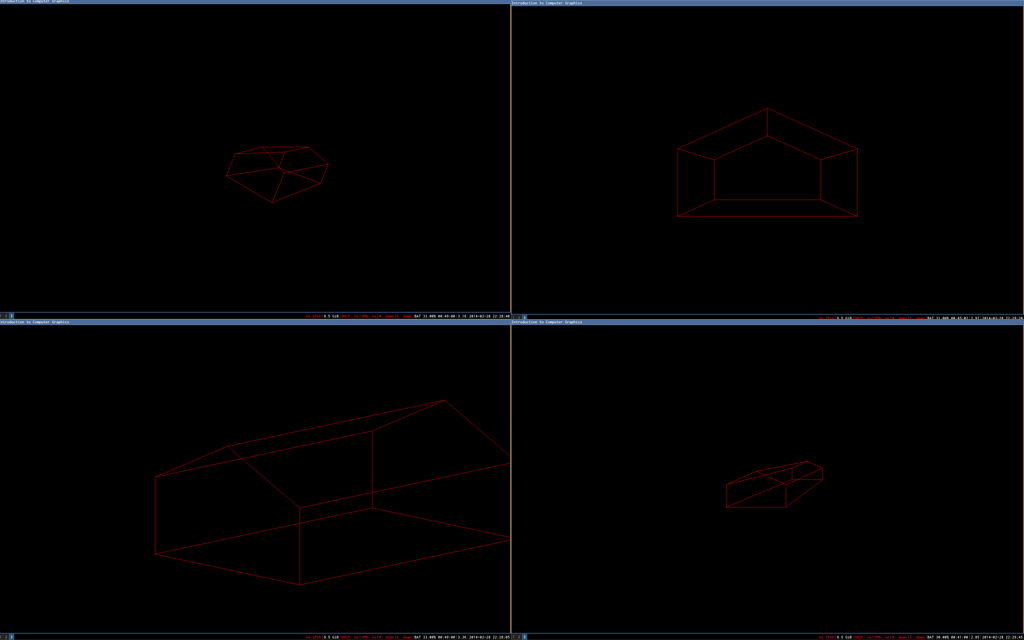
\includegraphics[scale=0.37]{figures/tests.jpg}
    \caption{Screenshots from the test program}
    \label{fig:screenshots}
\end{figure}

\end{document}

